%%%%%%%%%%%%%%%%%%%%%%%%%%%%%%%%%%%%%%%%%%%%%%%%%%%%%%%%%%%%%%%%%%%
\section{Étape 3: Extraire les noyaux et modéliser leur performance} \label{sec:methodo_step3}
%%%%%%%%%%%%%%%%%%%%%%%%%%%%%%%%%%%%%%%%%%%%%%%%%%%%%%%%%%%%%%%%%%%

Les deux premières étapes de la méthodologie s'intéressent à la recherche et à la caractérisation de nouvelles plateformes. La troisième étape concerne la modélisation des performances de l'application. Celle-ci est indépendante des deux premières étapes.


%%%%%%%%%%%%%%%%%
\subsection{Motivations et objectifs}
%%%%%%%%%%%%%%%%%


    En introduction de cette partie, nous avons rappelé la définition des \glspl{hotspot}. Ceux-ci sont particulièrement présents dans les applications de calcul haute performance et correspondent généralement aux \glspl{kernel} de calcul. Ces zones de codes possèdent un fort potentiel pour l'amélioration de la performance de l'application.  Si une application passe 99\% de ses cycles dans l'exécution d'une fonction, une amélioration d'un facteur 10 de celle-ci entraînera une amélioration du même facteur de l'application. Le travail du programmeur est donc d'identifier et d'accélérer ces parties en priorité.
    
    Les applications réelles utilisées en production dépassent souvent les dizaines de milliers de lignes de codes. Porter et optimiser la totalité d'une application serait complexe et contre-productif. De plus, la performance de chaque \gls{kernel} peut être limitée par des parties différentes du matériel (\gls{memorybound}, \gls{computebound}, etc), il est donc nécessaire de les porter individuellement sur différentes plateformes. 
    
    L'objectif de cette étape est d'identifier ces zones clés du code et de modéliser leur performance en fonction des performances de la bande passante mémoire (GB/s) ou du processeur (\gls{FLOPS}) en calculant leur intensité opérationnelle notée \gls{oikernel}. La majorité des codes étant limité par la performance de la mémoire, nous présentons un modèle de performance basé sur la performance du bus mémoire. 


%%%%%%%%%%%%%%%%%
\subsection{Identification des kernels}
%%%%%%%%%%%%%%%%%
    
    
    De nombreux travaux sont réalisés pour identifier et extraire les \glspl{kernel} d'une application \cite{castro2015cere, brunst2013custom}. L'outil de profilage \verb|perf| \cite{de2010new} permet d'extraire un sommaire de l'exécution d'une application en représentant son arbre d'appel. L'\autoref{perf_example} présente le résultat donné par la commande \verb|perf| lors de l'exécution du benchmark \verb|STREAM|. Cette commande permet de rapidement identifier les \glspl{kernel} et leur part de responsabilité dans le temps d'exécution de l'application. Elle nécessite d'exécuter l'application complète. Cependant, cet exercice ne doit être réalisé qu'une seule fois en début d'analyse pour identifier les zones de code sur lesquelles l'analyse doit se poursuivre.
    


\begin{lstlisting}[caption={Exemple d'utilisation de perf avec la commande \texttt{perf record  -g  -F 97} lors de l'exécution du benchmark \texttt{STREAM}. Le rapport d'exécution est obtenu avec la commande \texttt{perf report --stdio}.}, float, label={perf_example}]
# Samples: 116K of event 'cycles:ppp'
# Event count (approx.): 2744862582690
#
# Children      Self  Command          Shared Object       Symbol                                                                       
# ........  ........  ...............  .................. .......
    99.52%     0.00%  Stream.SKL.128   [unknown]           [k] 0000000000000000
            |          
             --99.52%--0
                       |          
                        --99.16%--0xadf96
                                  |
                                  |--25.35%--tuned_STREAM_Add   
                                  |--25.34%--tuned_STREAM_Triad
                                  |--20.36%--tuned_STREAM_Copy
                                  |--17.27%--tuned_STREAM_Scale
                                   --10.74%--main

\end{lstlisting}



%%%%%%%%%%%%%%%%%
\subsection{Modélisation de l'équilibre des kernels}
%%%%%%%%%%%%%%%%%
    
    Chaque \gls{kernel} peut être porté sur un accélérateur différent. Ainsi, ils doivent être analysés indépendamment les uns des autres. L'objectif de la modélisation est de comprendre les performances de l'application, et d'identifier si elles sont limitées par les performances du système mémoire \textbf{todo gls memory bound} ou par la capacité de calcul du processeur. La modélisation des performances permet ensuite de réduire le nombre d'architectures envisagées pour le portage de l'application. Cette étape permet d'éviter d'investir du temps et de l'argent dans des solutions inefficaces pour l'application étudiée. 
    
    Pour connaître lequel du système mémoire ou du processeur est le \gls{bottleneck}, le \verb|Roofline Model| (voir \autoref{sec:roofline}) peut être utilisé. Nous conseillons de construire le modèle à l'aide des caractéristiques mesurées lors de l'étape 2 (\gls{flopspeak} et \gls{memorypeak}) pour avoir une meilleure estimation des performances réellement atteignables. Pour établir le modèle d'un kernel, il est nécessaire de calculer l'intensité opérationnelle notée \gls{oikernel} et mesurée en $flop/byte$. Elle représente le nombre d'opérations réalisables par le processeur pour chaque donnée transférée depuis la mémoire. Ce calcul se fait à partir de la lecture du code source, ce qui motive le besoin d'identifier individuellement les \glspl{kernel}. 
    L'utilisation du modèle permet ensuite de visualiser les kernels ayant le plus grand potentiel d'amélioration de performance. 


%%%%%%%%%%%%%%%%%
\subsection{Simple Memory Model: Modélisation de la performance mémoire} \label{sec:smm}
%%%%%%%%%%%%%%%%%

    La majorité des codes HPC exécutée sur des architectures modernes voient leurs performances limitées par celle de la bande passante mémoire. Nous avons développé un modèle de performance simple, permettant de modéliser et valider les performances d'un code facilement. Pour réaliser cette modélisation, le développeur doit avoir accès au code source de l'application à porter. Pour un \gls{kernel} donné, il faut compter le nombre d'accès mémoire en distinguant les accès en lecture et ceux en écriture. Il est important de distinguer les accès en lecture et en écriture, car nous utiliserons leur ratio pour valider le bon comportement de la microarchitecture avec l'outil \verb|YAMB| (voir \autoref{sec:yamb}). En effet, nous montrons dans notre expérience que la saturation du bus mémoire n'est pas un indicateur suffisant pour conclure de l'efficacité ou non d'un code.
    
    Cette modélisation est faisable seulement si les \glspl{kernel} du code ont été identifiés, l'appliquer sur la totalité de l'application serait trop long. 
    Pour être appliqué à un kernel donné, il faut tout d'abord calculer la taille du jeu de données utilisé pour l'exécution, notée \texttt{DATA}$_\texttt{size}$. En lisant le code, il est alors possible de calculer la quantité de données minimale qui doit être transférée sur le bus mémoire. Grâce à l'étape 2, nous connaissons les performances maximales théoriques \gls{memorypeak} et réelle \gls{memorymax} de la microarchitecture. La durée optimale pour exécuter le kernel étudié peut alors être calculée (\autoref{eq:optimal}). Cette durée mesurée en seconde est notée \gls{tempsoptimal}. 
    
    \begin{equation}\label{eq:optimal}
        \texttt{TEMPS}_\texttt{optimal}\ = \frac{\texttt{DATA}_\texttt{size}}{\texttt{MEMORY}_\texttt{max}}
    \end{equation}

    
    Le modèle suppose que le code utilise un algorithme parfait (utilisation de la localité des données), que la compilation du code a été réalisée avec un compilateur parfait et qu'il est exécuté sur une plateforme parfaite. L'objectif n'est pas d'atteindre exactement cette performance, mais de s'en approcher le plus possible. Généralement, lorsqu'un défaut apparaît à un des niveaux énumérés précédemment, la performance s'éloigne radicalement de la performance optimale.
    
    




%%%%%%%%%%%%%%%%%
\subsection{Application des modèles Roofline et SMM}
%%%%%%%%%%%%%%%%%
    
    Dans l'\autoref{perf_example}, le profil de l'exécution du benchmark \verb|STREAM| comporte quatre fonctions utilisées pour stresser la mémoire par différent type d'accès. Nous choisissons arbitrairement de consacrer notre analyse sur un des quatre \glspl{kernel}: la fonction \textit{triad} dont le code peut être vu dans l'\autoref{code:triad}. Cette fonction est intéressante, car ce motif d'accès est très courant dans les applications HPC.
    
    
\begin{lstlisting}[language=c,caption=La fonction \textit{triad} du benchmark Stream utilise trois tableaux: deux en lecture et une en écriture,label={code:triad}, 
  basicstyle=\footnotesize, frame=tb,
  xleftmargin=.065\textwidth, xrightmargin=.065\textwidth]
for (j=0; j < STREAM_ARRAY_SIZE; j++)
    A[j] = B[j] + scalar * C[j];
\end{lstlisting}
        
        
    
    \subsubsection{Modèle du Roofline}
    %%%%%%%%%%%%%%%%%
        Lors de l'étape 1, nous avons mesuré la performance mémoire maximale atteignable \gls{memorymax} de 105 GB/s. L'utilisation du \verb|Kernel Generator| nous avait permis de mesurer une performance \gls{flopsmax} de 1372.78 GFlop/s, proche de la performance théorique de l'architecture. Ces deux mesures permettent de construire le \textit{toit} du modèle du Roofline présenté sur la \autoref{pic:Roofline_stream}.
        
        Pour évaluer les limitations du \gls{kernel} étudié, il est ensuite nécessaire de calculer son intensité opérationnelle notée \gls{oikernel}. Lors de chaque itération de boucle, le processeur doit charger 3 éléments en double précision, soit 24 bytes, correspondant aux tableaux $A$, $B$ et $C$ de l'\autoref{code:triad}. En effet, hors optimisation, une ligne de cache doit être chargée avant d'être écrite, même si aucune des données n'est utilisée en lecture par le processeur. À chaque itération de boucle, deux opérations doivent être réalisées, une addition et une multiplication. Cette fonction a donc une intensité arithmétique \gls{oikernel} $= \frac{2}{24} = 0.083$ flop/byte.
        Pour comparaison, les processeurs récents ont un ratio proche de $10\ flop/byte$. Cette simple modélisation montre le déséquilibre qu'il y a entre la performance de la mémoire et celle des processeurs. Elle permet de guider le choix de la plateforme sur laquelle cette fonction devra être portée. La \autoref{pic:Roofline_stream} montre l'application du Roofline à l'étude de la fonction \textit{triad} et au processeur étudié. Cette fonction ayant une faible intensité opérationnelle (\gls{oikernel}), ses performances théoriques mesurées en flop sont elles aussi très faibles.
        
        \begin{figure}
            \center
            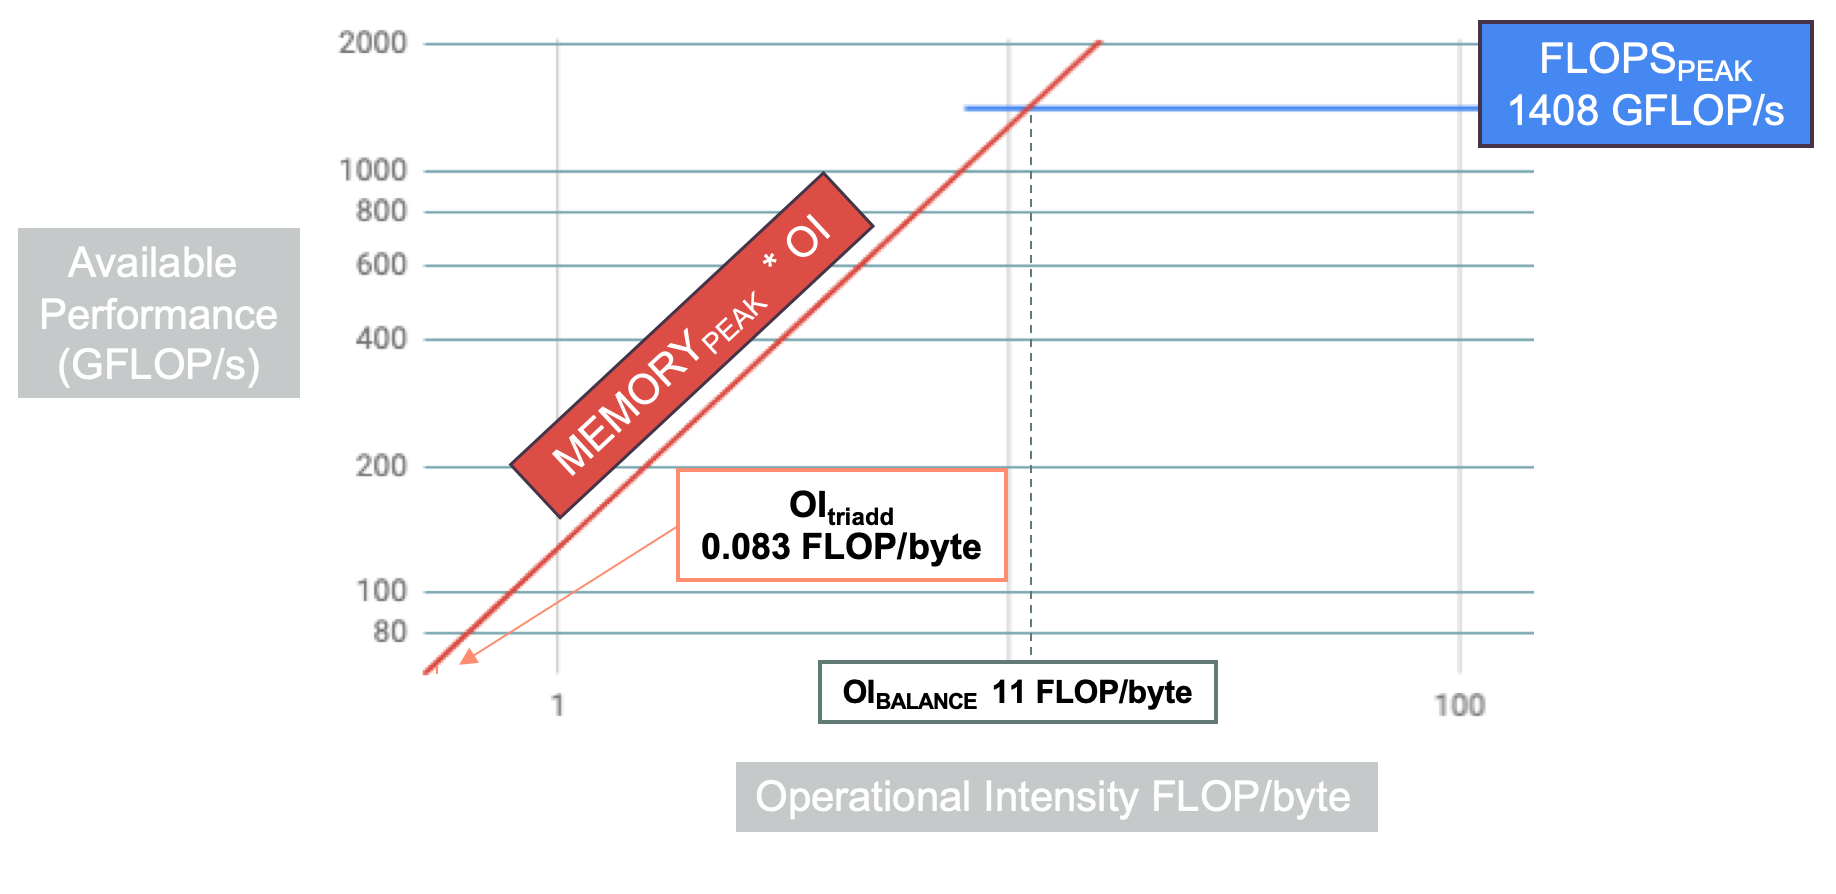
\includegraphics[width=14cm]{images/roofline_stream.png}
            \caption{\label{pic:Roofline_stream} Modèle du \textit{Roofline} appliqué à la fonction \textit{triad} du benchmark \textit{Stream} et un processeur Xeon Skylake 6148.}
        \end{figure}
    


\subsubsection{Application du Simple Memory Model} 
%%%%%%%%%%%%%%%%%
    L'analyse du noyau avec le modèle du Roofline indique que sur l'architecture ciblée, la performance du code sera limitée par la performance de la bande passante.
    Une fois assuré que les performances de l'application sont limitées par le système mémoire, le Simple Memory Model peut être appliqué. 
    
    Dans notre expérimentation, nous utilisons trois tableaux de 19.6 GB ($3 \times 10^9 \times sizeof(double)$). Pour une exécution optimale, le bus mémoire devrait être utilisé:
    \begin{itemize}
        \item pour la lecture des tableaux $B$ et $C$;
        \item pour l'écriture du tableau $A$.
    \end{itemize}
    Le trafic mémoire total serait alors de 58.8 GB. En utilisant les résultats mesurés lors de l'étape 2, on peut estimer le temps optimal pour l'exécution de cette fonction: \gls{tempsoptimal} $= \frac{58.8}{128} = 0.56$ seconde. 
    Cette modélisation nous permet de projeter la performance optimale sur une architecture sans avoir à exécuter le code sur celle-ci. La valeur \gls{tempsoptimal} permet ensuite de vérifier que les performances maximales de l'architecture sont atteintes. Dans le cas contraire, cette valeur peut être utilisée pour quantifier le gain de performance pouvant être obtenu grâce à l'optimisation du code.